\section{Empirical Evaluation}
In this section, we make an empirical evaluation of our algorithm by performing a set of experiments on the synthetic data set, and several real world data sets.

\subsection{Comparison Methods}
In order to evaluate the effectiveness of our algorithm, we choose three time series similarity algorithms and four correlation coefficient in our experiment. 

For the three similarity algorithm, we choose L1-Distance, L2-Distance \cite{han2011data}, and DTW-Distance \cite{muller2007dynamic}. 
And for the three statistic correlation algorithm, we choose Pearson correlation coefficient\cite{nagelkerke1991note}, two ranking based correlation coefficients: The Kendall rank correlation \cite{kendall1938new}, and Spearman's rank correlation \cite{pirie1988spearman}.

In the rest of this subsection, we briefly introduce the three similarity measures and the three Correlation measures.

\subsubsection{Similarity Measures}

Given a two time series 
$X=(x_1,x_2,...,x_m),Y=(y_1,y_2,...,y_m)$, where $m$ is the length of the time series.

The L1-distance is denoted as follow:
\begin{equation}
L_1(X,Y) = \sum_{1}^{m}|x_i-y_i|
\end{equation}

The L2-distance is denoted as follow:
\begin{equation}
L_2(X,Y) = \sqrt{\sum\nolimits_{1}^{m}|x_i-y_i|^2}
\end{equation}

The third similarity measure we used is DTW distance \cite{muller2007dynamic}, which is a famous time series similarity measure.

In order to introduce the DTW distance, we firstly construct an $m-by-m$ matrix $W$, where the $(i-{th},j-{th})$ element of the matrix $W$. The DTW distance is to find a path through the matrix that minimizes the total cumulative distance between $X$ and $Y$. 
So, the optimal path is the path that minimize the warping cost:

\begin{equation}
DTW(X,Y) = \min { \sqrt{\sum\nolimits_{k=1}^{K}w_k}}
\end{equation}
where, $w_k$ belongs to the $k-{th}$ element of a warping path $P$, which is a contiguous set of elements that represent a mapping between $X$ and $Y$.

\subsubsection{Correlation Measures}

In this subsection, we introduce three widely used correlation measures between time series: Pearson Correlation \cite{pearson1904mathematical}, Kendall rank correlation \cite{kendall1938new}, and Spearman's rank correlation \cite{pirie1988spearman}.

The Pearson correlation coefficient, can be calculated as follow:

\begin{equation*}
Pearson(X,Y)=\frac{cov(X,Y)}{\sigma_X\sigma_Y}=\frac{E[(X-\mu_X)(Y-\mu_Y)]}{\sigma_X\sigma_Y}
\end{equation*}
where $cov$ is the covariance, $\sigma_X$ is the standard deviation of $X$, $\mu_X$ is the mean of $X$ and $E[*]$ denotes the expectation.

The Kendall rank correlation \cite{kendall1938new} is defined as follow:
\begin{equation*}
Kendall(X,Y)=\frac{N_c - N_d}{m(m-1)/2}
\end{equation*}
where $N_c$ is the number of concordant pairs, and $N_d$ is the number of discordant pairs, and $m$ is the dimension of the time series.
For any pair $(x_i,y_i)$ and $x_j,y_j$, where $i \neq j$, are said to be concordant both $x_i > x_j$ and $y_i > y_j$, or $x_i < x_j$ and $y_i < y_j$. Otherwise, they are discordant.

The Spearman's rank correlation \cite{pirie1988spearman} is defined as follow:
\begin{equation*}
Spearman(X,Y)=1 - \frac{6\sum d^2_i}{n(n^2-1)}
\end{equation*}
where $d_i$ is defined as the difference between the ranks of $x_i$ and $y_i$.

\subsection{Evaluation Strategy}
In order to evaluate both the correctness and efficiency of our method, we design two tasks using our measure and other measures: Time Series Clustering Task, and Time Series Top-k Search Task. In the rest of this subsection, we will brief introduce these two tasks in details.

\subsubsection{Clustering Task}

In order to evaluate the performance of our correlation coefficient, we design a clustering task. 
In this task, we use the Hierarchical Clustering \cite{han2011data} to evaluate the performance. Hierarchical Clustering is very sensitive to the distance measure. So, the clustering performance can directly illustrate the effectiveness of our method compared with other methods.

Two evaluation methods are used for testing the clustering result: Accuracy \cite{han2011data}, which is calculated as the percentage of target objects clustered into the correct clusters. The clustering accuracy ($r$) is defined as
\[
r = \frac{\sum\nolimits_{i=1}^{k}a_i}{n}
\]
where $a_i$ is the number of data objects occurring both in $i$th cluster and its corresponding true class, and $n$ is the number of time series.

Normalized Mutual Information (NMI) \cite{han2011data}, which is one of the most popular evaluation methods to evaluate the quality of clustering results. The normalized mutual information of two clustering result is defined as follow:
\[
NMI(X,Y) = \frac{I(X;Y)}{\sqrt{H(X)H(Y)}}
\]
where $X$ and $Y$ are vectors containing cluster labels for all the target objects, $I(X;Y)$ denotes the mutual information\cite{han2011data} of these two vector, $H(X)$ and $H(Y)$ are the marginal entropies\cite{han2011data}. 
Both accuracy and NMI are in the range of 0 to 1, and a higher value indicates a better clustering result in terms of ground truth.

\subsubsection{Top-K Searching Task}

In this work, we propose to use LSH scheme to do fast search. So, we design a top-k search task for by using different measures.

For the change based correlation measure, we use our proposed LSH search scheme. For the other similarity or correlation measures. We use naive based search. The step of naive based method is: (1) calculate all the distance between the query item and the items in the data set. (2) Ranking all the items based on the distance calculated in first step. (2) Return top k items. Naive based search can get the best search result for each measure.

We compute precision and recall \cite{powers2011evaluation} to evaluate all the top-k search result.
If the Searched time series is in the same cluster of the query time series, we regard it as a relevant items, and vice verse. We range the $K$ from $1$ to the cluster size. 

For each top-k Nearest Neighbors search, the precision can be calculated as follow:
\[Precision =\frac{relevant~item}{K} \]
and the recall can be calculated as follow:
\[
Precision =\frac{relevant~item}{Relevant~Cluster~Size} 
\]

\subsection{Effectiveness Study on Synthetic Dataset}

In this section, we introduce the experiment on the synthetic Dataset.
We first brief describe the synthetic dataset, and then show the experimental result of each tasks on this data sets by using different measures.

\subsubsection{The Synthetic Dataset}

Synthetic data set is very useful for evaluating algorithms and functions for data mining and machine learning models\cite{han2011data}. The steps of generating this synthetic data is showed as follow:

\begin{description}
  \item[Step 1] randomly generate $10000$ time series with two patterns of time series: (1) Periodical Pattern, (2) Linear Pattern. The length of each time series is $5000$. 
  \item[Step 2] Add white noise and correlated noise randomly \cite{han2011data} on each time series.
  \item[Step 3] Random shuffle all the $10000$ time series and Divide these $10000$ time series into $5$ groups.
  \item[Step 4] Add change randomly into $5$ groups, within same group, the change times are same, with different groups the change time are different. Seven different types of changes are added randomly into each time series, the seven change types are showed in Table.\ref{Tab:ChangeType}.
\end{description}

\begin{table}[t]
\caption{\textbf{Change Types in the Synthetic Data}}
\centering
\begin{tabular}{|c|}
\hline Change Type \\
\hline Mean Change \\
\hline Variance Change\\
\hline Frequency Change $+$ Variance Change\\
\hline Mean Change $+$ Frequency Change \\
\hline Frequency Change $+$ Variance Change\\
\hline Mean Change $+$ Frequency Change $+$ Variance Change\\
\hline
\end{tabular}
\label{Tab:ChangeType}
\end{table}

After obtaining these $10000$ time series with five groups.
In order to test both the efficiency and effectiveness of change based correlation coefficient. 
We choose four sub-set from these time series. 
We make the data set size from small to large, and also the time series length from short to long. The four sub dataset is showed in Table.\ref{Tab:SDataScale}. 

\begin{table}[t]
\caption{Summery of Synthetic Data}
\centering

\begin{tabular}{|c|c|c|}
\hline DataSet &  Data Size & Time Series Length\\
\hline Synthetic-T0 & 1000 & 800 \\
\hline Synthetic-T1 & 1000 & 5000 \\
\hline Synthetic-T2 & 10000 & 800 \\
\hline Synthetic-T3 & 10000 & 5000 \\
\hline
\end{tabular}
\label{Tab:SDataScale}
\end{table}


\begin{table*}
\caption{Clustering Performance on Synthetic Data Set}
\centering
\renewcommand{\arraystretch}{1.2}
\begin{tabular}{ccccccccc} 
\toprule[2pt] 
%\hline
Dataset & Measure & Proposed & $L1$ & $L2$ & DTW & Pearson & Kendall & Spearman \\
\toprule[1.5pt] 
\multirow{2}*{\centering{Sythetic-T0}}
     & Accuracy & $\boldsymbol{.854\pm.032}$ & $.241\pm.098$ & $.281\pm.012$ & $.230\pm.061$ & $.309\pm.140$ & $.353\pm.026$ & $.297\pm.036$ \\
\cline{2-9}
     & NMI & $\boldsymbol{.808\pm.034}$ & $.026\pm.067$ & $.076\pm.023$ & $.028\pm.075$ & $.140\pm.55$ & $.395\pm.015$ & $.150\pm.088$ \\
\toprule[1.2pt] 
\multirow{2}*{\centering{Sythetic-T1}}
     & Accuracy & $\boldsymbol{.838\pm.025}$ & $.247\pm.026$ & $.262\pm.032$ & $.283\pm.012$ & $.240\pm.018$ & $.374\pm.067$ & $.341\pm.067$ \\
\cline{2-9}
     & NMI & $\boldsymbol{.701\pm.030}$ & $.003\pm.062$ & $.057\pm.043$ & $.064\pm.036$ & $.046\pm.084$ & $.404\pm.023$ & $.230\pm.042$ \\
\toprule[1.2pt] 
\multirow{2}*{\centering{Sythetic-T2}}
     & Accuracy & $\boldsymbol{.806\pm.029}$ & $.254\pm.066$ & $.263\pm.080$ & $.304\pm.022$ & $.388\pm.024$ & $.384\pm.032$ & $.502\pm.182$ \\
\cline{2-9}
     & NMI & $\boldsymbol{.889\pm.012}$ & $.028\pm.042$ & $.056\pm.056$ & $.054\pm.032$ & $.303\pm.064$ & $.394\pm.052$ & $.450\pm.049$ \\
\toprule[1.2pt] 
\multirow{2}*{\centering{Sythetic-T3}}
     & Accuracy & $\boldsymbol{.856\pm.077}$ & $.225\pm.028$ & $.229\pm.034$ & $.284\pm.062$ & $.454\pm.032$ & $.454\pm.032$ & $.454\pm.032$ \\
\cline{2-9}
     & NMI & $\boldsymbol{.891\pm.017}$ & $.021\pm.040$ & $.041\pm.043$ & $.086\pm.038$ & $.454\pm.032$ & $.454\pm.032$ & $.454\pm.032$ \\
\bottomrule[1.5pt] 
\end{tabular}
\label{Tab:ClusRes}
\end{table*}
%\begin{figure*}[t]
%\centering
%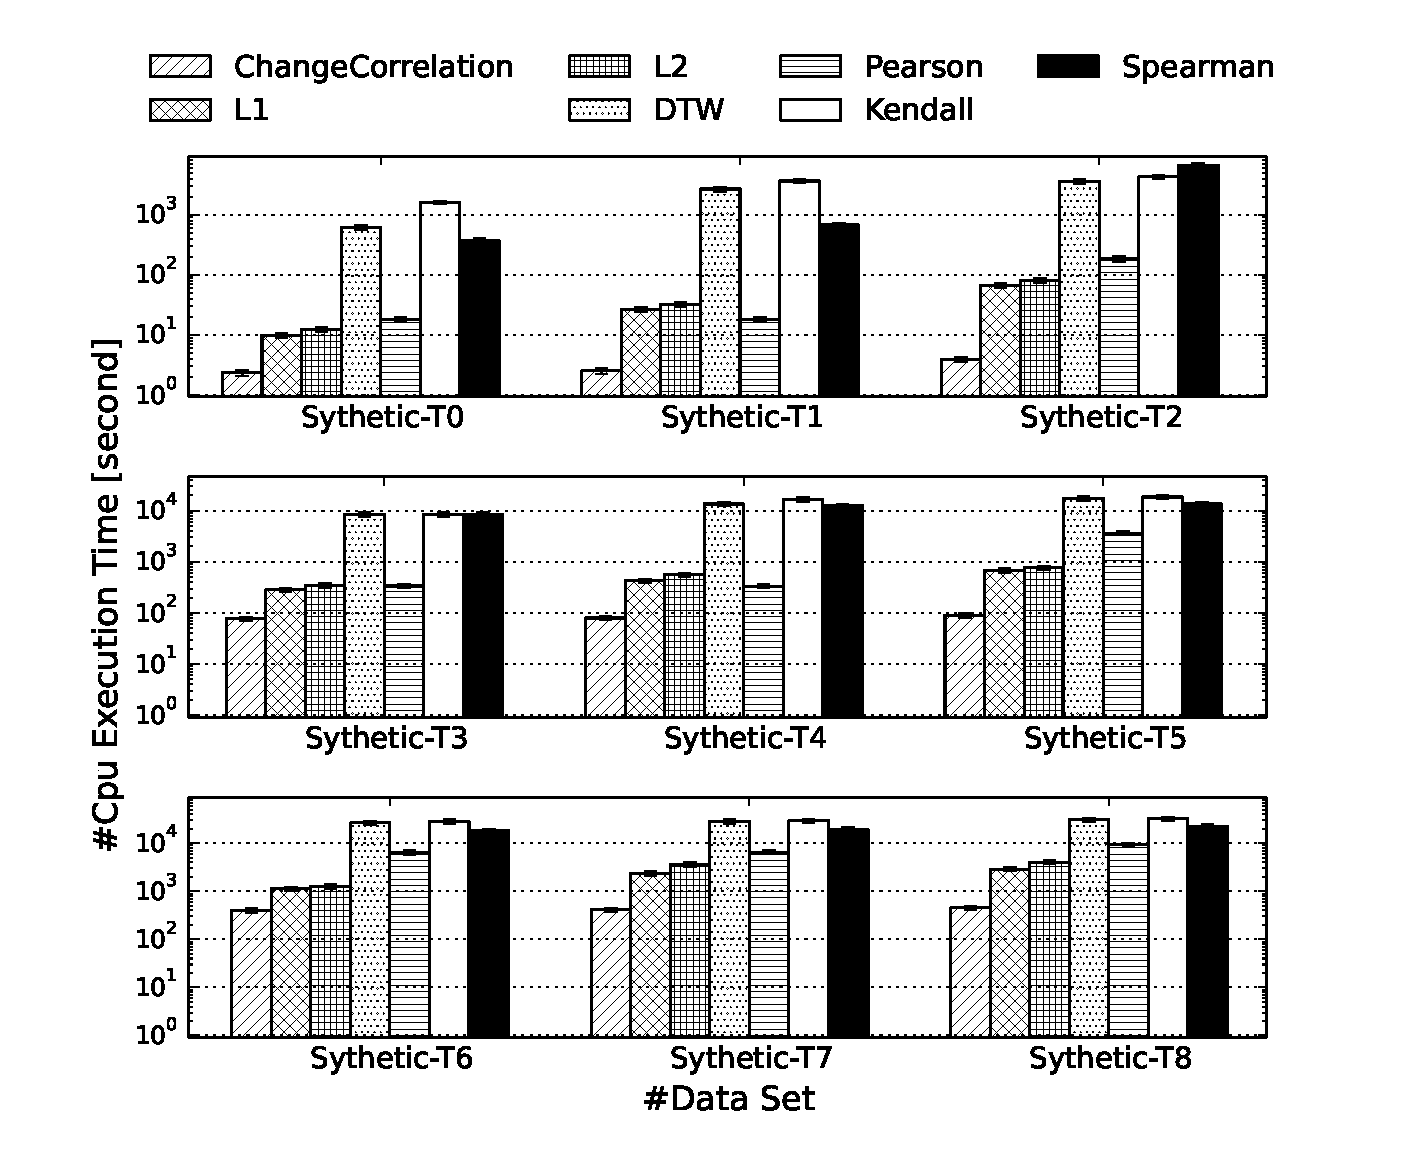
\includegraphics[width=0.8\textwidth]{SythClusPerf.eps}
%\caption{Top-k Nearest Neighbor Search}
%\label{Fig:ClusPerf}
%\end{figure*}

%\begin{figure*}
%\centering
%\subfigure{%
%\includegraphics[width=0.45\textwidth]{VaryDataSize.eps}
%}\hspace{0.001em}
%\subfigure{%
%\includegraphics[width=0.45\textwidth]{VaryDataDimension.eps}
%}\hspace{0.001em}
%\caption{Efficiency by varying data size and dimension size}
%\label{fig:NNPerf}
%\end{figure*}



\subsubsection{Clustering task on Synthetic Data}

The clustering task result on these four synthetic data are showed in Table.\ref{Tab:ClusRes}.

From Table.\ref{Tab:ClusRes}, we can see that, for the change correlation coefficient, the clustering result performance is better for the high dimensional data set.
This is because that for high dimensional time series data, the proposed coefficient can extract more change information from the time series data and also make more accurate evaluation of the correlation. 
From this point of view, change based correlation is more suitable for the high dimensional time series data set.
On the other hand, Change based correlation can obtain more accuracy results in different dataset compared with both the similarity method and the correlation coefficient. So, the result of clustering show the effectiveness of our coefficient.

\subsubsection{Top-k Searching task on Synthetic Data}

\begin{figure*}[t]
\centering

\subfigure{%
\includegraphics[width=0.41\textwidth]{PRC3.eps}
}\hspace{0.001em}
\subfigure{%
\includegraphics[width=0.41\textwidth]{PRC2.eps}
}\hspace{0.001em}
\subfigure{%
\includegraphics[width=0.41\textwidth]{PRC1.eps}
}\hspace{0.001em}
\subfigure{%
\includegraphics[width=0.41\textwidth]{PRC0.eps}
}
%
\caption{Precision Recall Curve for Different Algorithms}
\label{fig:NNPreRe}
\end{figure*}

\begin{table}
\caption{Query Time for Top-10 Search}
\centering
\renewcommand{\arraystretch}{1.2}
\begin{tabular}{ccccc} 
\toprule[2pt] 
%\hline
\multirow{2}*{\centering{Measure}}
     & \multicolumn{4}{c}{Data Set} \\
\cline{2-5}
     & T0\footnote{``T0" denotes Synthetic-T0} & T1 & T2 & T3\\
\toprule[1.2pt] 
     Proposed & $0.004$ & $0.01$ & $0.0033$ & $0.08$\\
\hline
     L1 & $0.01$ & $0.1$ & $0.13$ & $0.85$\\
\hline
     L2& $0.02$ & $0.15$ & $0.15$ & $1.05$\\
\hline
     DTW & $0.7$ & $107.59$ & $15.82$ & $0.20$\\
\hline
     Pearson & $0.22$ & $0.29$ & $2.04$ & $0.85$\\
\hline
     Kendall & $2.80$ & $55.39$ & $26.53$ & $2.07$\\
\hline
     Spearman & $0.4$ & $1.81$ & $3.87$ & $1.18$\\
\toprule[1.2pt] 
\end{tabular}
\label{Tab:Synthetic}
\end{table}

The plots for all the four datasets are shown in Figure.\ref{fig:NNPreRe}. We can clearly see that our proposed Change-based Correlation method gives significantly higher precision recall curves than other similarity and correlation methods. In addition the results are consistent across datasets. 

Table.\ref{Tab:Synthetic} shows the Execution time of the clustering task on each data set. From the result, we can see that change based correlation performed much faster than other algorithms. 


\subsection{Effectiveness Study on Real Datasets}

In this section, we will compare the proposed algorithm with the baseline algorithms on two real data sets.

\subsubsection{Electrocardiogram Data set}

The first real world dataset is ECG (Electrocardiogram) time series data set. This data set comes from the the UCR time series Data set Archive \cite{UCRArchive}. We choose four ECG data set there as showed in Table. \ref{Tab:ECGData}. And the ground truth comes from the UCR data set itself.

For the clustering task, we use the Hierarchical Clustering \cite{han2011data} to evaluate the performance as before. 
From Table.\ref{Tab:ECGClus}, we can see that, for the change based correlation can obtain more accuracy results in these four ECG data set compared with both the similarity method and the correlation coefficient. So, the result of clustering show the effectiveness of our coefficient.

For the Top-K searching task. The plots for all the four ECG dataset datasets are shown in Figure.\ref{fig:ECGPRC}.
We can clearly see that our proposed Change-based Correlation method gives significantly higher precision recall curves than other similarity and correlation methods. In addition the results are consistent across datasets. This demonstrate the effectiveness of change-based correlation coefficient and the corresponding LSH search algorithm.

Table.\ref{Tab:ECGTime} shows the Execution time of the top-k searching task on each ECG data set. From the result, we can see that change based correlation performed much faster than other algorithms. 

\begin{table*}[t]
\caption{Summary of the Four ECG Data Set}
\centering

\begin{tabular}{|c|c|c|c|}
\hline Data Set & \centering Data Size & Time Series Length & Class Numver\\
\hline CinC_ECG_torso & \centering 1380 & 1639 & 4\\
\hline ECGFiveDays & \centering 861 & 136 & 2\\
\hline TwoLeadECG & \centering 1139 & 82 & 2\\
\hline ECG5000 & \centering 4500 & 140 & 5\\
\hline
\end{tabular}
\label{Tab:ECGData}
\end{table*}

\begin{table*}[t]
\caption{Clustering Performance on Synthetic ECG Data Set From UCR Time Series Archive}
\centering
\renewcommand{\arraystretch}{1.2}
\begin{tabular}{ccccccccc} 
\toprule[2pt] 
%\hline
Dataset & Measure & Proposed & $L1$ & $L2$ & DTW & Pearson & Kendall & Spearman \\
\toprule[1.5pt] 
\multirow{2}*{\centering{CinC_ECG_torso}}
     & Accuracy & $\boldsymbol{.839\pm.011}$ & $.667\pm.068$ & $.557\pm.012$ & $.610\pm.061$ & $.531\pm.140$ & $.507\pm.019$ & $.504\pm.013$ \\
\cline{2-9}
     & NMI & $\boldsymbol{.489\pm.019}$ & $.236\pm.035$ & $.019\pm.023$ & $.010\pm.075$ & $.280\pm.55$ & $.150\pm.015$ & $.049\pm.012$ \\
\toprule[1.2pt] 
\multirow{2}*{\centering{EGG_5000}}
     & Accuracy & $\boldsymbol{.538\pm.025}$ & $.247\pm.026$ & $.262\pm.032$ & $.283\pm.012$ & $.240\pm.018$ & $.374\pm.067$ & $.341\pm.067$ \\
\cline{2-9}
     & NMI & $\boldsymbol{.401\pm.030}$ & $.003\pm.062$ & $.057\pm.043$ & $.064\pm.036$ & $.046\pm.084$ & $.404\pm.023$ & $.230\pm.042$ \\
\toprule[1.2pt] 
\multirow{2}*{\centering{TwoLeadECG}}
     & Accuracy & $\boldsymbol{.810\pm.029}$ & $.504\pm.066$ & $.538\pm.080$ & $.620\pm.022$ & $.528\pm.064$ & $.531\pm.052$ & $.519\pm.049$ \\
\cline{2-9}
     & NMI & $\boldsymbol{.680\pm.012}$ & $.081\pm.042$ & $.043\pm.056$ & $.137\pm.032$ & $.047\pm.064$ & $.062\pm.052$ & $.074\pm.049$ \\
\toprule[1.2pt] 
\multirow{2}*{\centering{ECGFiveDays}}
     & Accuracy & $\boldsymbol{.832\pm.077}$ & $.502\pm.028$ & $.527\pm.034$ & $.615\pm.062$ & $.506\pm.032$ & $.547\pm.032$ & $.519\pm.032$ \\
\cline{2-9}
     & NMI & $\boldsymbol{.765\pm.017}$ & $.002\pm.040$ & $.002\pm.043$ & $.361\pm.038$ & $.075\pm.032$ & $.023\pm.032$ & $.086\pm.032$ \\
\bottomrule[1.5pt] 
\end{tabular}
\label{Tab:ECGClus}
\end{table*}

\begin{figure*}[t]
\centering
\subfigure{%
\includegraphics[width=0.45\textwidth]{PRCCinCECGtorso.eps}
}\hspace{0.001em}
\subfigure{%
\includegraphics[width=0.45\textwidth]{PRCECG5000.eps}
}\hspace{0.001em}
\subfigure{%
\includegraphics[width=0.45\textwidth]{PRCTwoLeadECG.eps}
}\hspace{0.001em}
\subfigure{%
\includegraphics[width=0.45\textwidth]{PRCECGFiveDays.eps}
}\hspace{0.001em}
\caption{Precision Recall Curve (higher is better). We compare Change based correlation coefficient with other methods.}
\label{fig:ECGPRC}
\end{figure*}

\begin{table*}
\caption{Query Time for Top-10 Search}
\centering
\renewcommand{\arraystretch}{1.2}
\begin{tabular}{ccccc} 
\toprule[2pt] 
%\hline
\multirow{2}*{\centering{Measure}}
     & \multicolumn{4}{c}{Data Set} \\
\cline{2-5}
     & CinCECGtorso & ECG5000 & TwoLeadECG & ECGFiveDays\\
\toprule[1.2pt] 
     Proposed & $0.005$ & $0.02$ & $0.003$ & $0.01$\\
\hline
     L1 & $0.04$ & $0.07$ & $0.01$ & $0.028$\\
\hline
     L2& $0.05$ & $0.078$ & $0.11$ & $0.030$\\
\hline
     DTW & $12.55$ & $0.59$ & $0.025$ & $0.20$\\
\hline
     Pearson & $0.31$ & $0.15$ & $0.21$ & $0.85$\\
\hline
     Kendall & $10.67$ & $0.39$ & $0.39$ & $2.07$\\
\hline
     Spearman & $0.82$ & $0.23$ & $0.28$ & $1.18$\\
\toprule[1.2pt] 
\end{tabular}
\label{Tab:ECGTime}
\end{table*}

\subsubsection{HPC Thread Time Series Data set}

The second real world dataset is collected from the HPCToolKit during three HPC task running. 

\begin{description}
  \item[Single PC] \hfill \\
  Single PC is a small toy execution task that execute on a single PC and small number of threads (20). In this datasets, there are two types of threads: Main Thread and Child Thread. We use the label of Main Thread and Child Thread as ground truth information.
  \item[MADNESS] \hfill \\ MADNESS\footnote{https://en.wikipedia.org/wiki/MADNESS} is a high level software sofware environment for Scientific Simulation. We use this environment to simulation several Scientific calculations, and generate 264 threads.
  The same of Single PC dataset, there are two types of thread: Main Thread and Child Thread. We also use them as ground truth information.
  \item[Earth Environment Simulation] \hfill \\ 
  This data set is collected from an earth Environment Simulation task. In this task, there are a several of simulation programs, including Oceans Simulation Programs, Weather simulation Programs, and several other simulation programs. The Oceans Simulation Program, and the Weather simulation Program are correlated with each other due to high frequency data transformation and communication. So the ground truth in this data is defined that programs with high frequency communications are having the same label.
  \ldots
\end{description}

We perform both clustering task and top-k search task on these three data set.

From Table.\ref{Tab:HPCClus}, we can see that, for the change based correlation can obtain more accuracy results in the two HPC Thread Time series data set compared with both the similarity method and the correlation coefficient. While we can see that DTW method can also get high accuracy, this because in data set, most of the thread in same class often in same state. However, as we said before, in some cases, thread in same class, the state can be different.

The precision recall curve for the HPC Thread TIme Series data is showed in Figure \ref{fig:HPCPRC}. We can clearly see that our proposed Change-based Correlation method gives higher precision recall curves than other similarity and correlation methods. Also, DTW method can get good result too. In addition the results are consistent across datasets. This demonstrate the effectiveness of change-based correlation coefficient and the corresponding LSH scheme.

\begin{table}
\caption{Summary of the HPC Time Series Data Set}
\centering

\begin{tabular}{|c|c|c|}
\hline Data Set & \centering Data Size & Time Series Length \\
\hline Single PC & \centering 24 & 4096 \\
\hline MADNESS & \centering 264 & 32768 \\
\hline Environment Simulation & \centering 312 & 16384 \\
\hline
\end{tabular}
\label{Tab:HPCData}
\end{table}

\begin{table}[t]
\caption{Query Time for Top-10 Search}
\centering
\renewcommand{\arraystretch}{1.2}
\begin{tabular}{cccc} 
\toprule[2pt] 
%\hline
\multirow{2}*{\centering{Measure}}
     & \multicolumn{3}{c}{Data Set} \\
\cline{2-4}
     & SinglePC & MADNESS & Earth \\
\toprule[1.2pt] 
     Proposed & $0.02$ & $0.16$ & $0.10$ \\
\hline
     L1 & $0.18$ & $1.02$ & $0.53$ \\
\hline
     L2& $0.48$ & $5.27$ & $2.79$ \\
\hline
     DTW & $21.83$ & $2537.21$ & $898.31$ \\
\hline
     Pearson & $0.35$ & $2.45$ & $1.20$ \\
\hline
     Kendall & $9.25$ & $1324.26$ & $536.32$ \\
\hline
     Spearman & $1.25$ & $315.45$ & $112.56$ \\
\toprule[1.2pt] 
\end{tabular}
\label{Tab:HPCTime}
\end{table}

\begin{table*}[t]
\caption{Clustering Performance on Synthetic ECG Data Set From UCR Time Series Archive}
\centering
\renewcommand{\arraystretch}{1.2}
\begin{tabular}{ccccccccc} 
\toprule[2pt] 
%\hline
Dataset & Measure & Proposed & $L1$ & $L2$ & DTW & Pearson & Kendall & Spearman \\
\toprule[1.5pt] 
\multirow{2}*{\centering{Single PC}}
     & Accuracy & $\boldsymbol{.917\pm.011}$ & $.835\pm.068$ & $.815\pm.012$ & $.870\pm.061$ & $.501\pm.140$ & $.527\pm.019$ & $.514\pm.013$ \\
\cline{2-9}
     & NMI & $\boldsymbol{.889\pm.019}$ & $.736\pm.035$ & $.719\pm.023$ & $.860\pm.075$ & $.380\pm.55$ & $.350\pm.015$ & $.349\pm.012$ \\
\toprule[1.2pt] 
\multirow{2}*{\centering{MADNESS}}
     & Accuracy & $\boldsymbol{.938\pm.025}$ & $.927\pm.026$ & $.922\pm.032$ & $.935\pm.012$ & $.457\pm.018$ & $.474\pm.067$ & $.541\pm.067$ \\
\cline{2-9}
     & NMI & $\boldsymbol{.861\pm.030}$ & $.853\pm.062$ & $.857\pm.043$ & $.864\pm.036$ & $.346\pm.084$ & $.404\pm.423$ & $.230\pm.442$ \\
\toprule[1.2pt] 
\multirow{2}*{\centering{Simulation}}
     & Accuracy & $\boldsymbol{.921\pm.021}$ & $.802\pm.026$ & $.420\pm.032$ & $.435\pm.012$ & $.857\pm.018$ & $.464\pm.067$ & $.531\pm.067$ \\
\cline{2-9}
     & NMI & $\boldsymbol{.831\pm.030}$ & $.803\pm.062$ & $.537\pm.043$ & $.504\pm.036$ & $.786\pm.084$ & $.202\pm.423$ & $.330\pm.442$ \\
\toprule[1.2pt] 
\end{tabular}
\label{Tab:HPCClus}
\end{table*}

\begin{figure}[t]
\centering
\subfigure{%
\includegraphics[width=0.45\textwidth]{PRCSinglePC.eps}
}\hspace{0.001em}
\subfigure{%
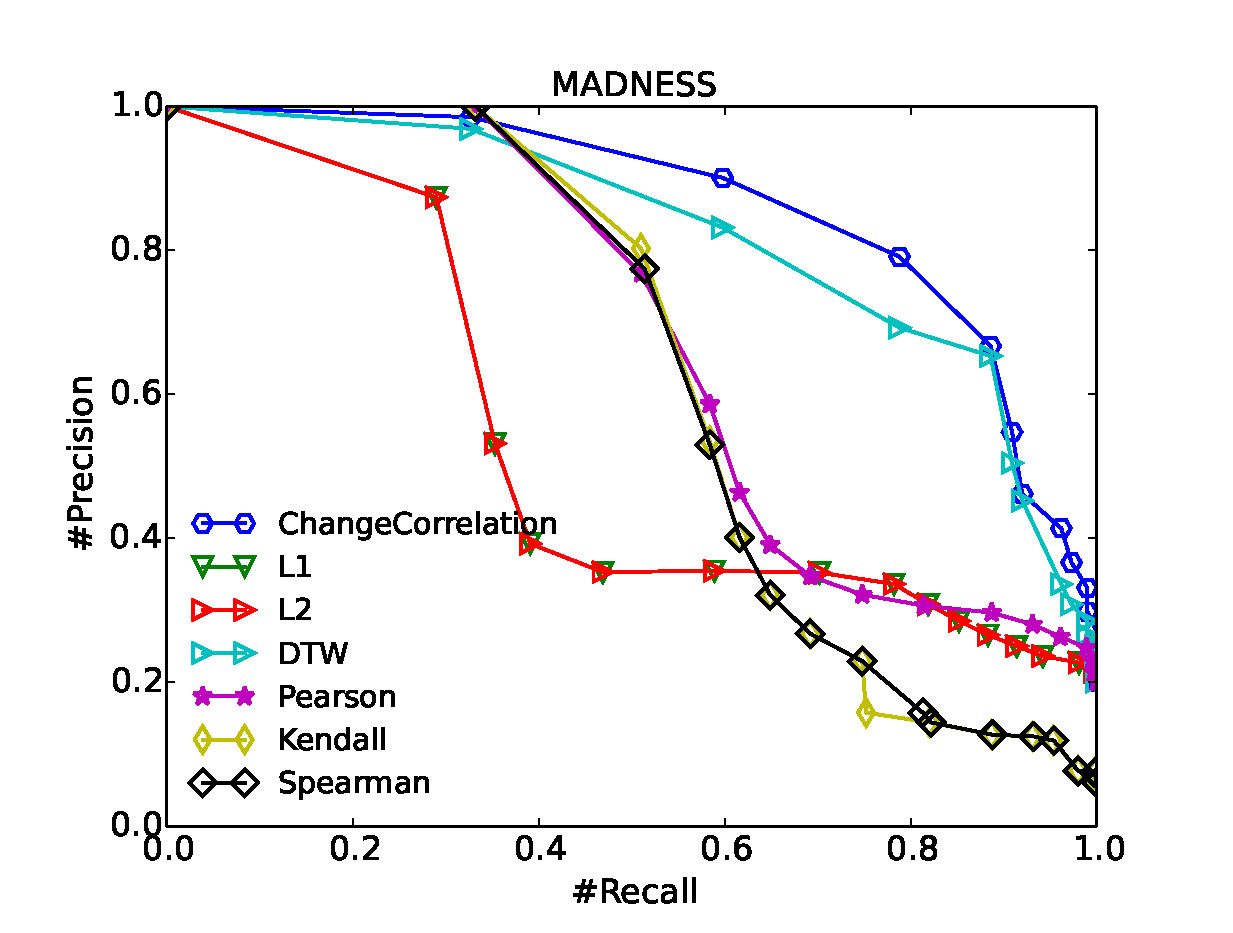
\includegraphics[width=0.45\textwidth]{PRCMADNESS.eps}
}\hspace{0.001em}
\subfigure{%
\includegraphics[width=0.45\textwidth]{PRCEnvironment.eps}
}\hspace{0.001em}
\caption{Precision Recall Curve (higher is better). We compare Change based correlation coefficient with other methods.}
\label{fig:HPCPRC}
\end{figure}


